\section{Design}

\subsection{Component Division}

The first question that has to be answered is whether or not it makes sense to divide the bootware component into two or more cooperating components, i.e. a server client division or a similar structure.
As described in \autoref{related:ondemand} on page \pageref{related:ondemand}, the proposed architecture initially only envisioned one bootware component.
This architecture was expanded with the introduction of the provisioning manager, as described in \autoref{related:dynamic} on page \pageref{related:dynamic}.
We will now discuss the viability of these architectures.

\subsubsection{Single Local Component}

\begin{figure}[!htbp]
	\centering
	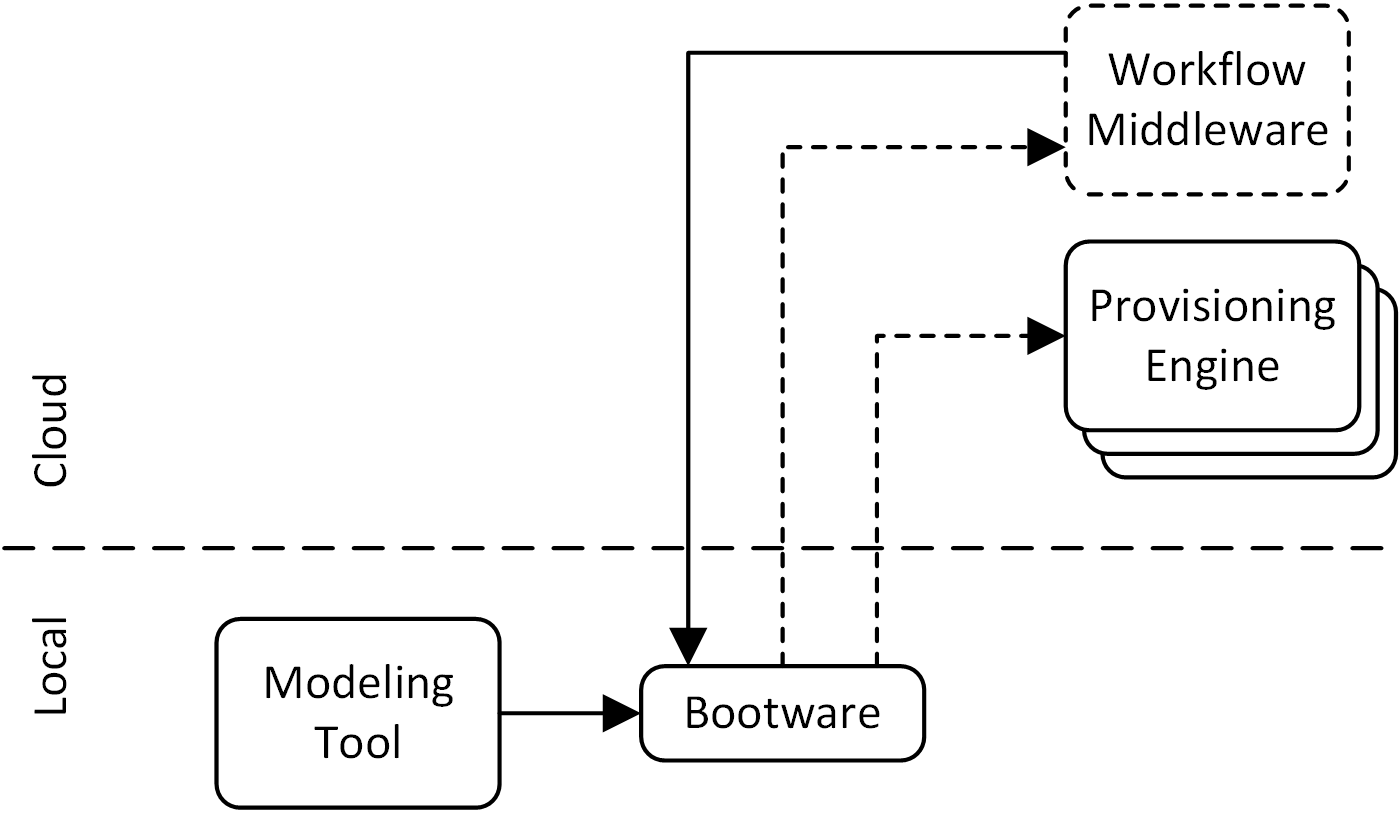
\includegraphics[resolution=600]{design/assets/simple_local}
	\caption{Simplified overview of the single local component architecture}
	\label{image:single_local}
\end{figure}

First we consider the simplest case: A single local component.
In this scenario, all provisioning processes are initiated from a component installed locally on the users machine, alongside or as part of the workflow modeler.

The advantages of this architecture lie in its simplicity.
Only one component has to be created and managed.
There is no possible overlap in functionality, as in a 2-tier architecture (see \autoref{design:division:2tier}.
Communication between multiple bootware components doesn't have to be considered.

The disadvantages are caused by the component being local.
Since all the functionality is concentrated in one component, it can become quite large and complicated, is is one thing that should be avoided according to the requirements.
A much bigger problem however is the remote communication happening in this scenario.
All calls to the bootware component from the ESB of the workflow middleware would leave the remote environment.
Also, all calls from the bootware component to the provisioning engines would enter the remote environment.
This type of split communication can be costly and slow \textcolor{red}{(add source/description)}.

\subsubsection{Single Remote Component}

\begin{figure}[!htbp]
	\centering
	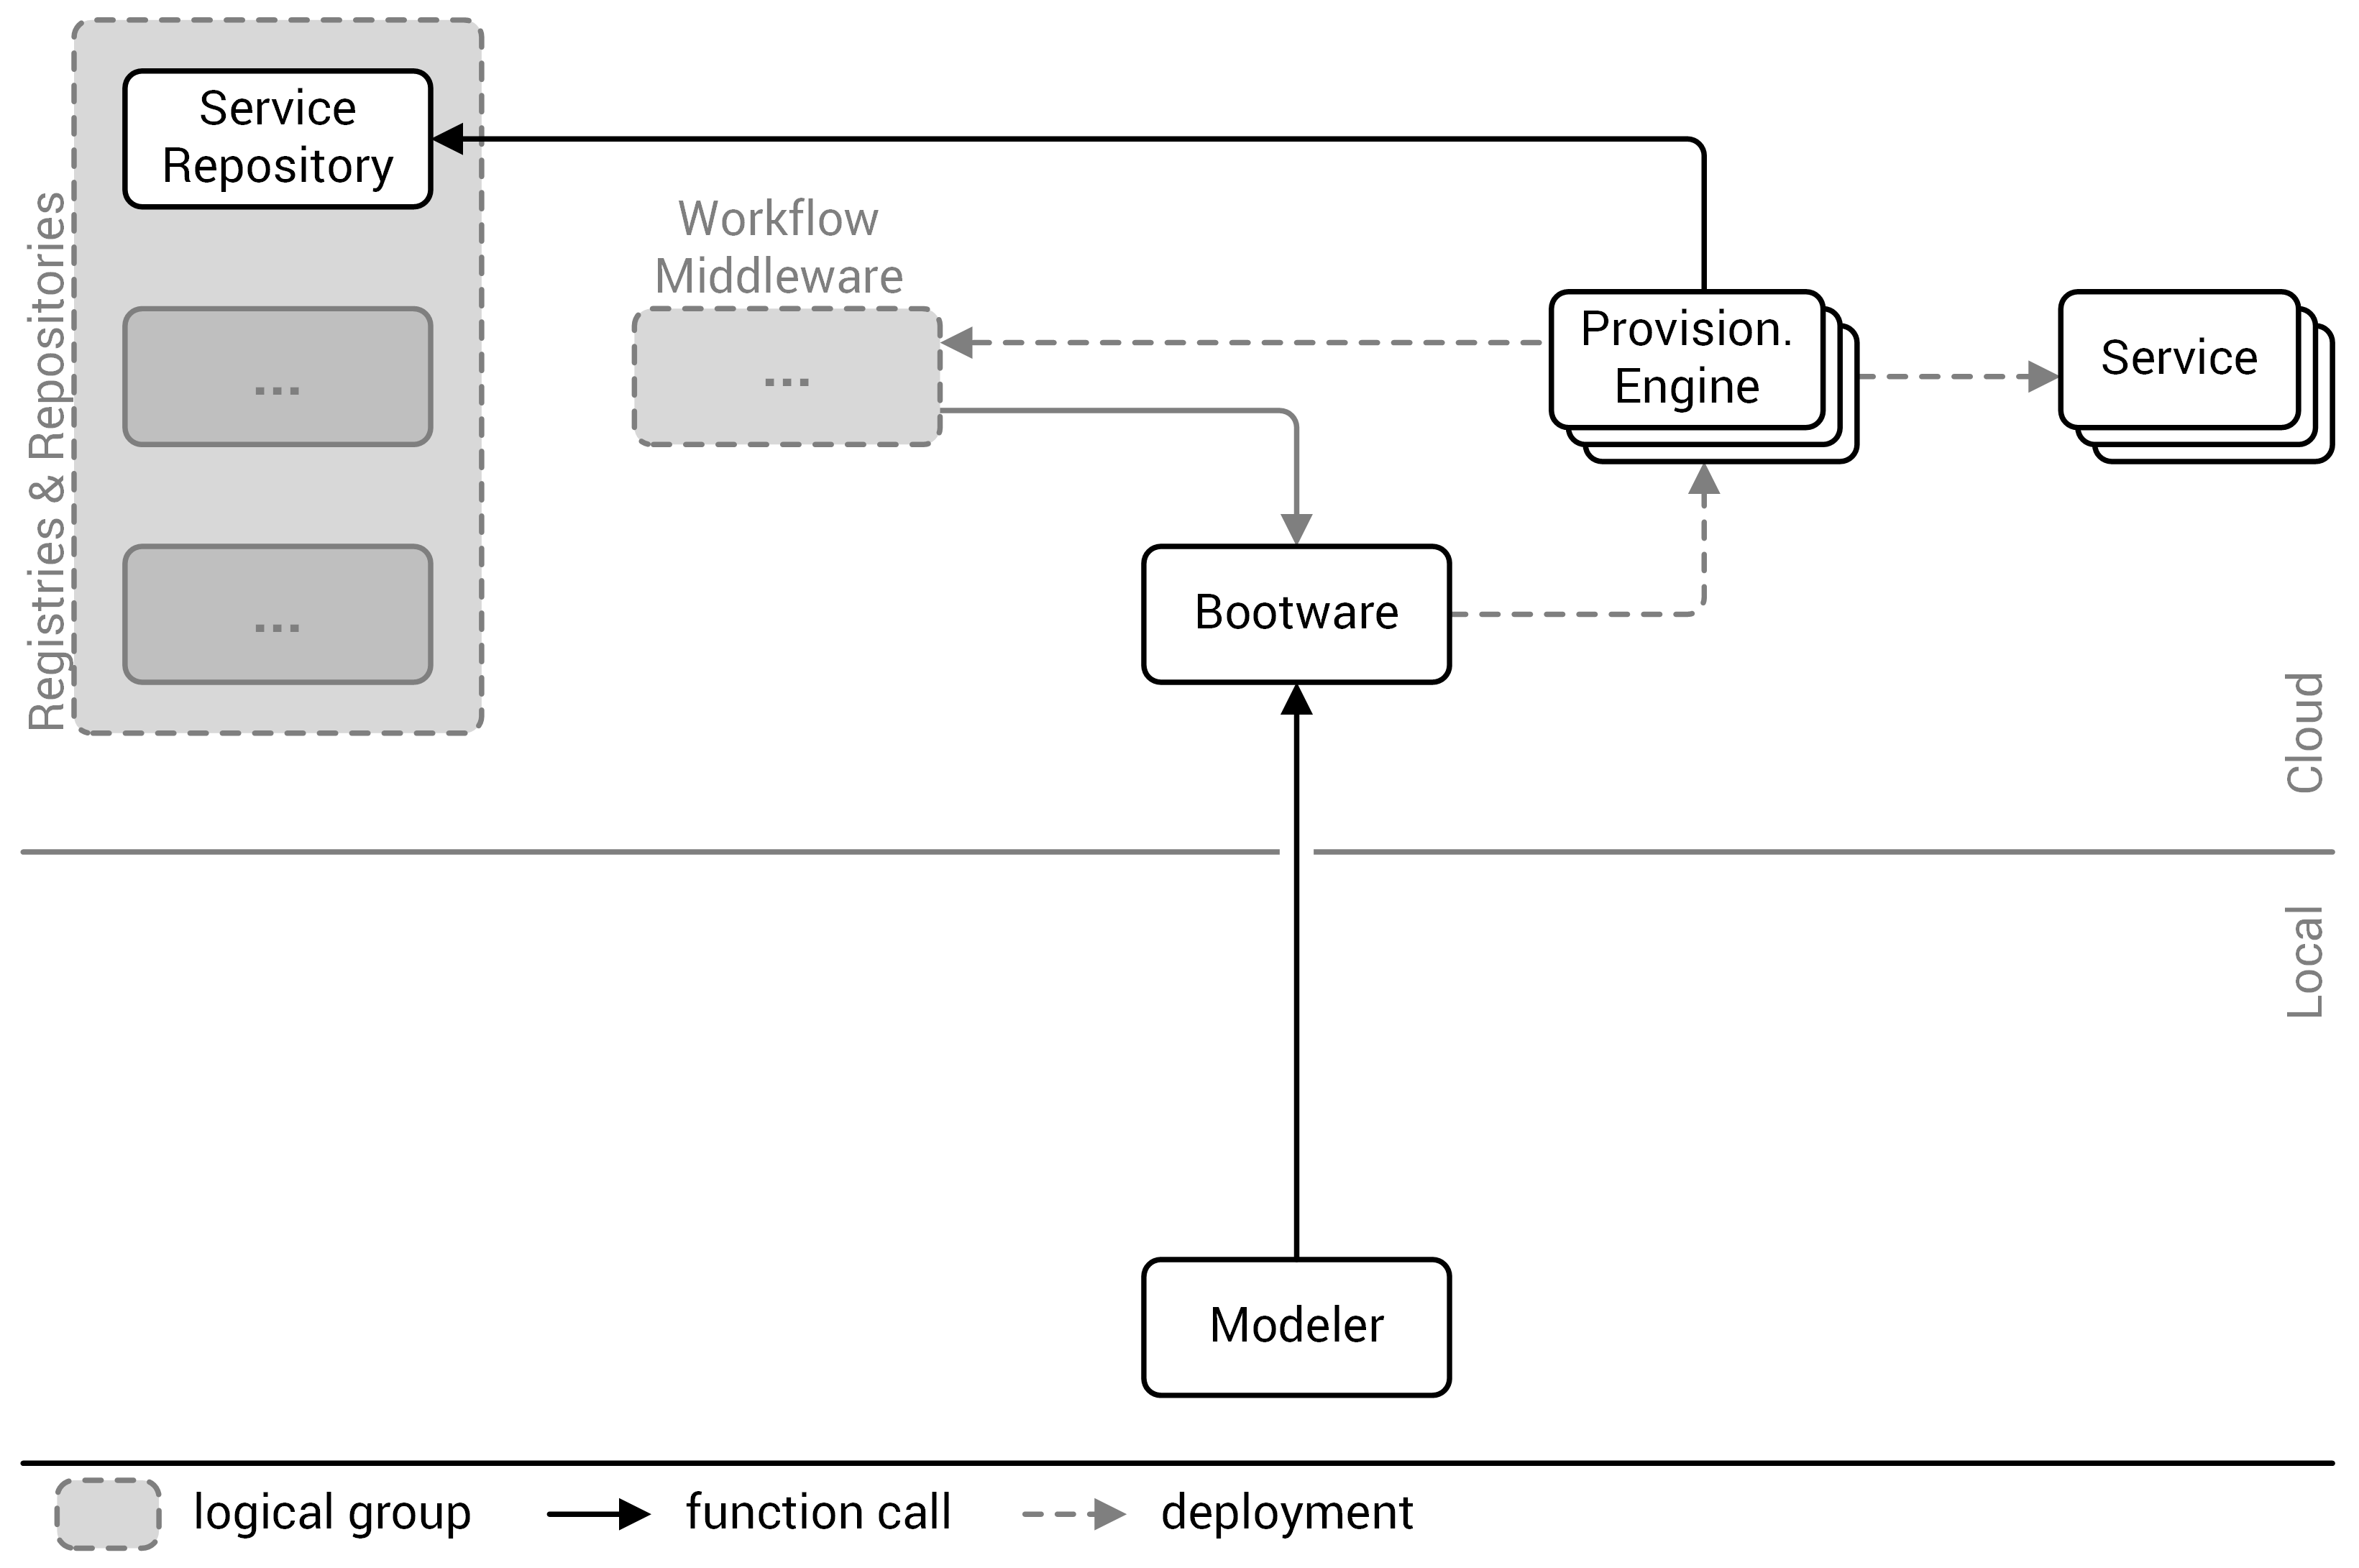
\includegraphics[resolution=600]{design/assets/simple_remote}
	\caption{Simplified overview of the single remote component architecture}
	\label{image:single_remote}
\end{figure}

The next obvious choice is to put the single bootware component into a remote environment, where the disadvantages of local to remote communication would disappear.

However, this creates a new problem.
We don't know where exactly to put the bootware component.
Since one requirement is that multiple cloud environments should be supported, it's possible that the bootware component is not located anywhere near the cloud environment where it should provision further components.
The communication problem of the single local bootware component still exist.

Another problem is that now we would have to manage some sort of load balancing and the bootware component would have to support multiple tenancy or be stateless, or otherwise every user needs its own remote instance.
The first case would further complicate the design and implementation of the bootware component.
The second case would increase monetary and management costs.

\subsubsection{2-Tier Architecture}
\label{design:division:2tier}

\begin{figure}[!htbp]
	\centering
	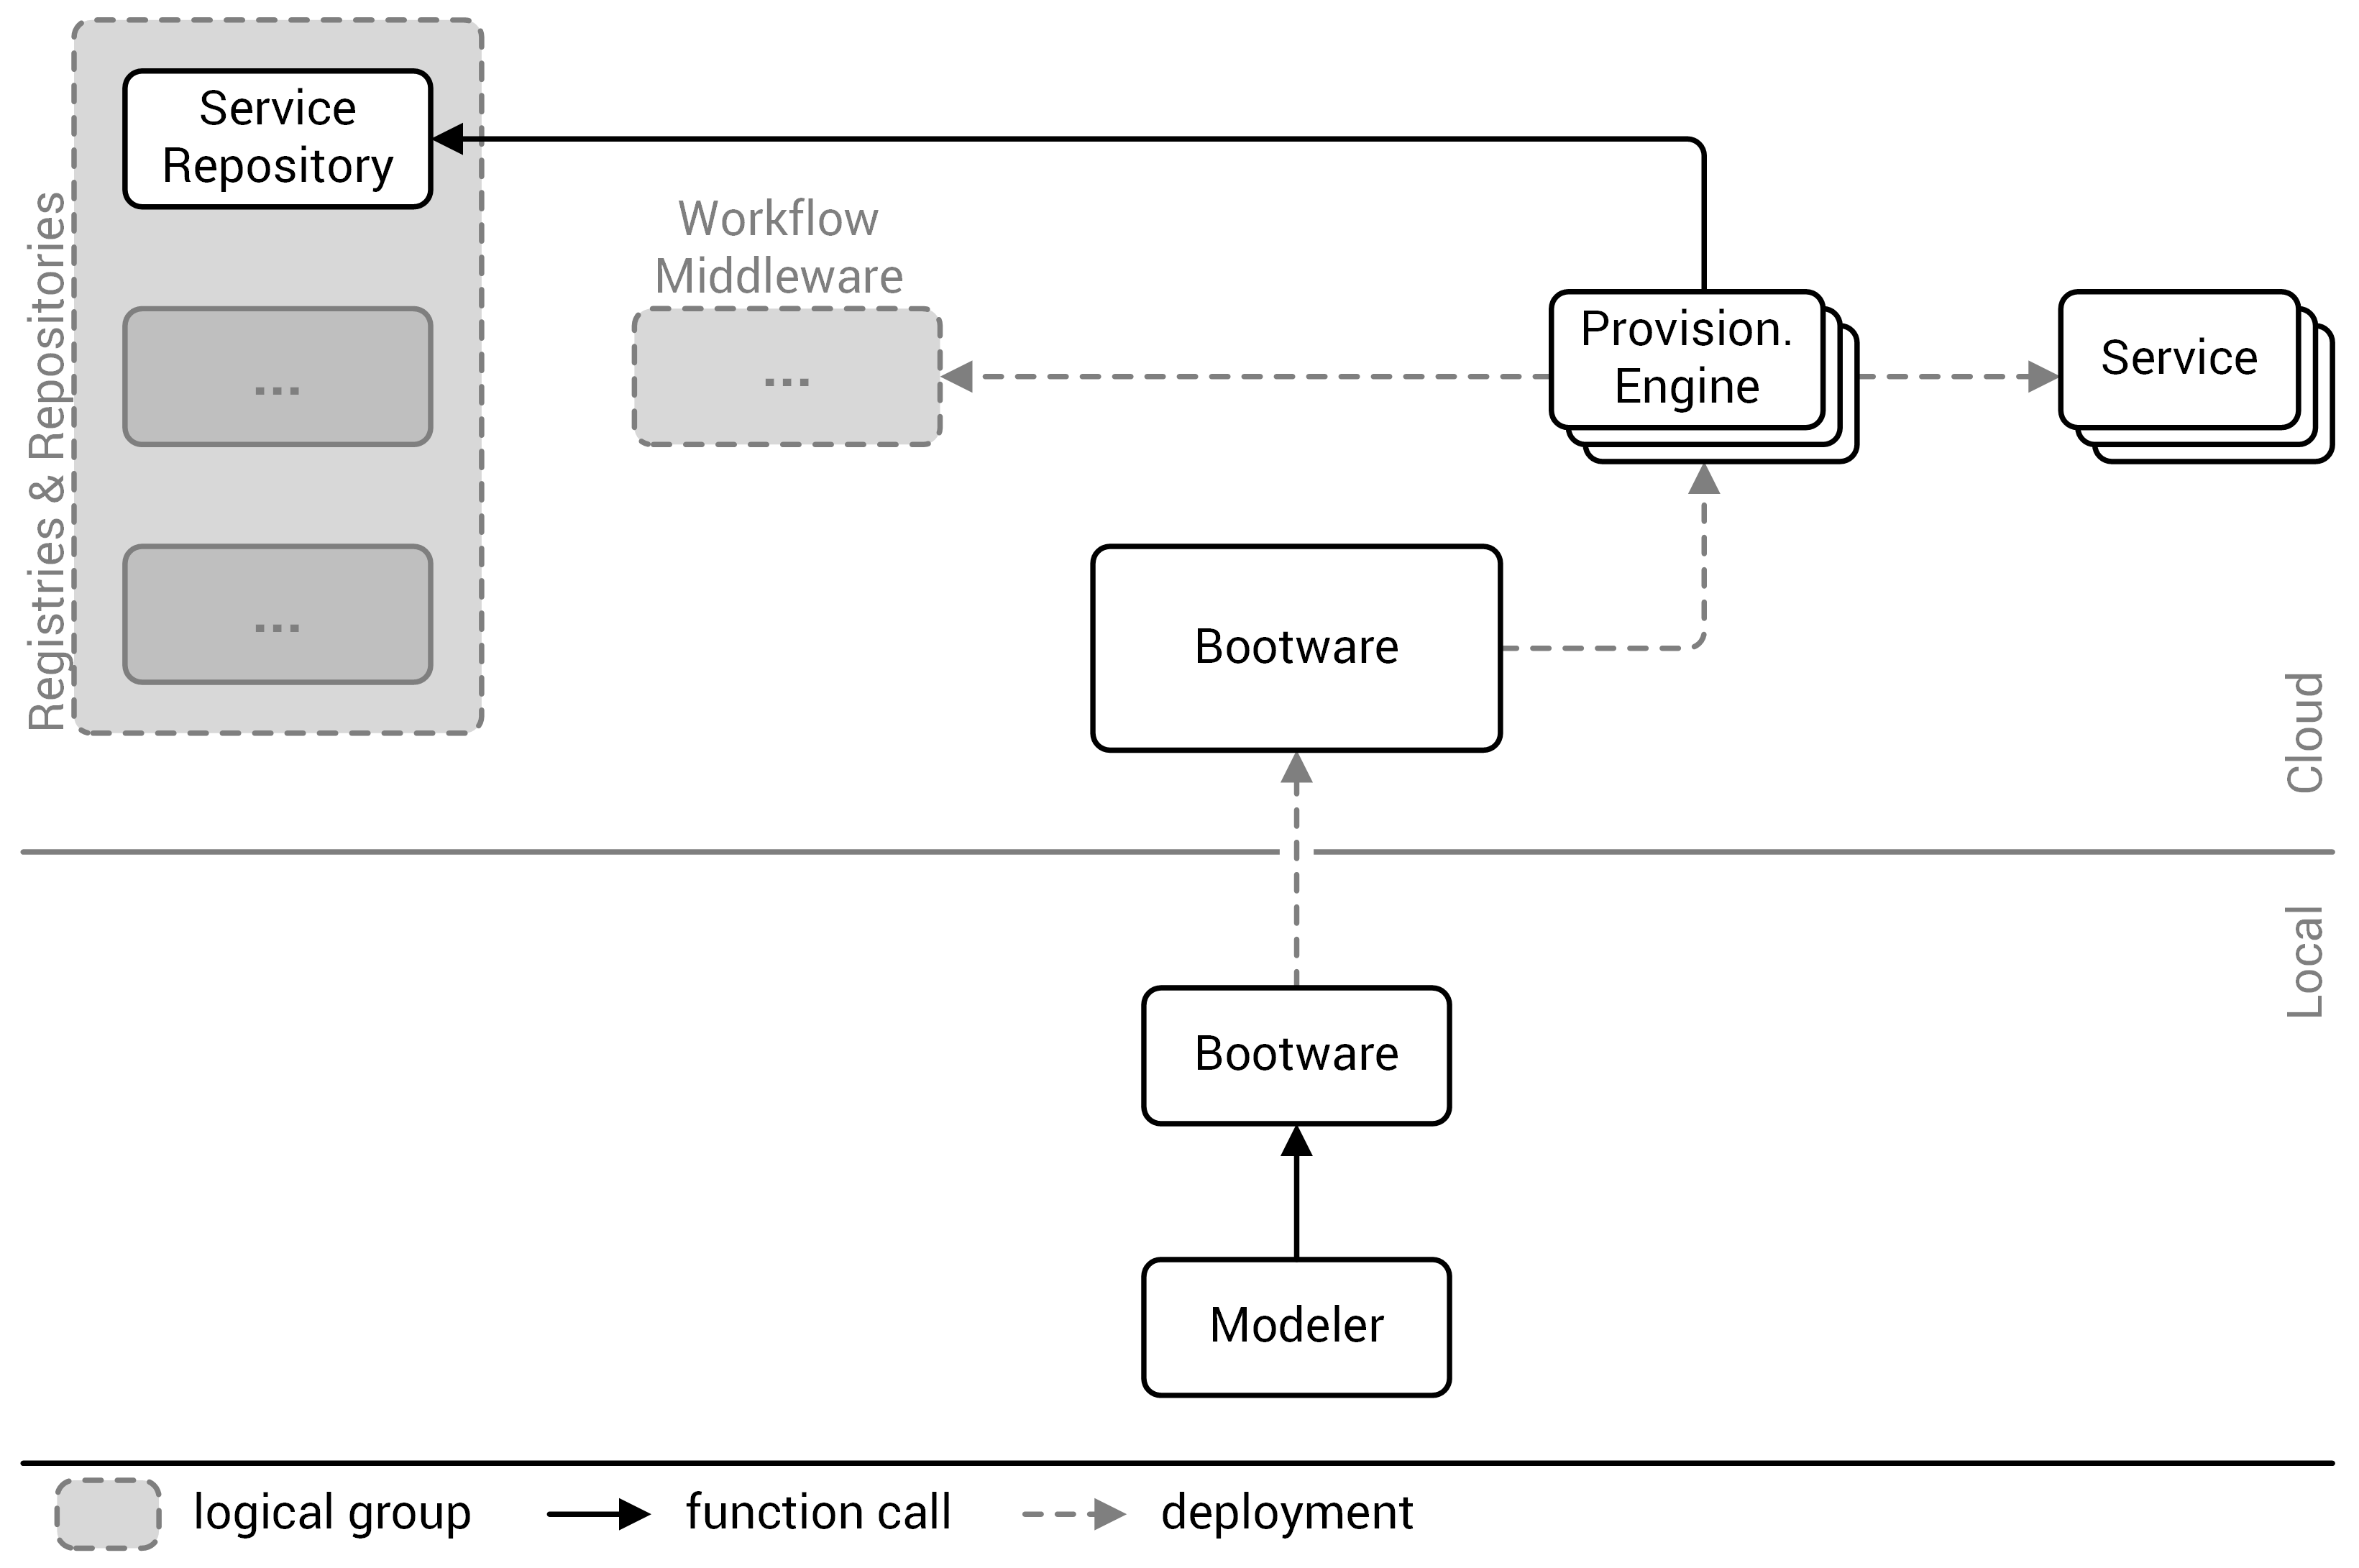
\includegraphics[resolution=600]{design/assets/simple_2_tier}
	\caption{Simplified overview of the 2-tier architecture}
	\label{image:2_tier}
\end{figure}

Next, we take a look at a 2-tier architecture, where the bootware is divided into two components.
On the local side we have a small and simple component which has mainly one function: To provision the larger second part of the bootware in a remote environment near to the environment, where other components will be provisioned later.

This eliminates the problems of a single bootware component.
We can now keep the local part as simple as possible and make the remote part as complicated as it has to be.
We now also can position the remote component close to other remote components to minimize local/remote communication and the problems resulting of it.

But we also introduce new problems.
For one, we now have duplicate functionality between the two components.
Both components have to know how to provision a component into multiple cloud environments.
The local component has to be able to put its remote counterpart into any cloud environment.
The remote component has to be able to provision other components into the same environment in which it runs (ideally, to minimize costs).
Since itself can be located in any cloud environment, it has to be able to do this in any cloud environment.
Independent from this, it has to be able to provision to any environment that the user/service package chooses.
But this problem can be solved by using a plugin architecture, which allows both components to use the same plugins.
We discuss plugins in detail in \autoref{design:extensibility}.

A second problem which we can't avoid but can solve is the communication which is now necessary between the different parts of the bootware.
More on this in \autoref{design:communication}

\subsubsection{Cloning}

\begin{figure}[!htbp]
	\centering
	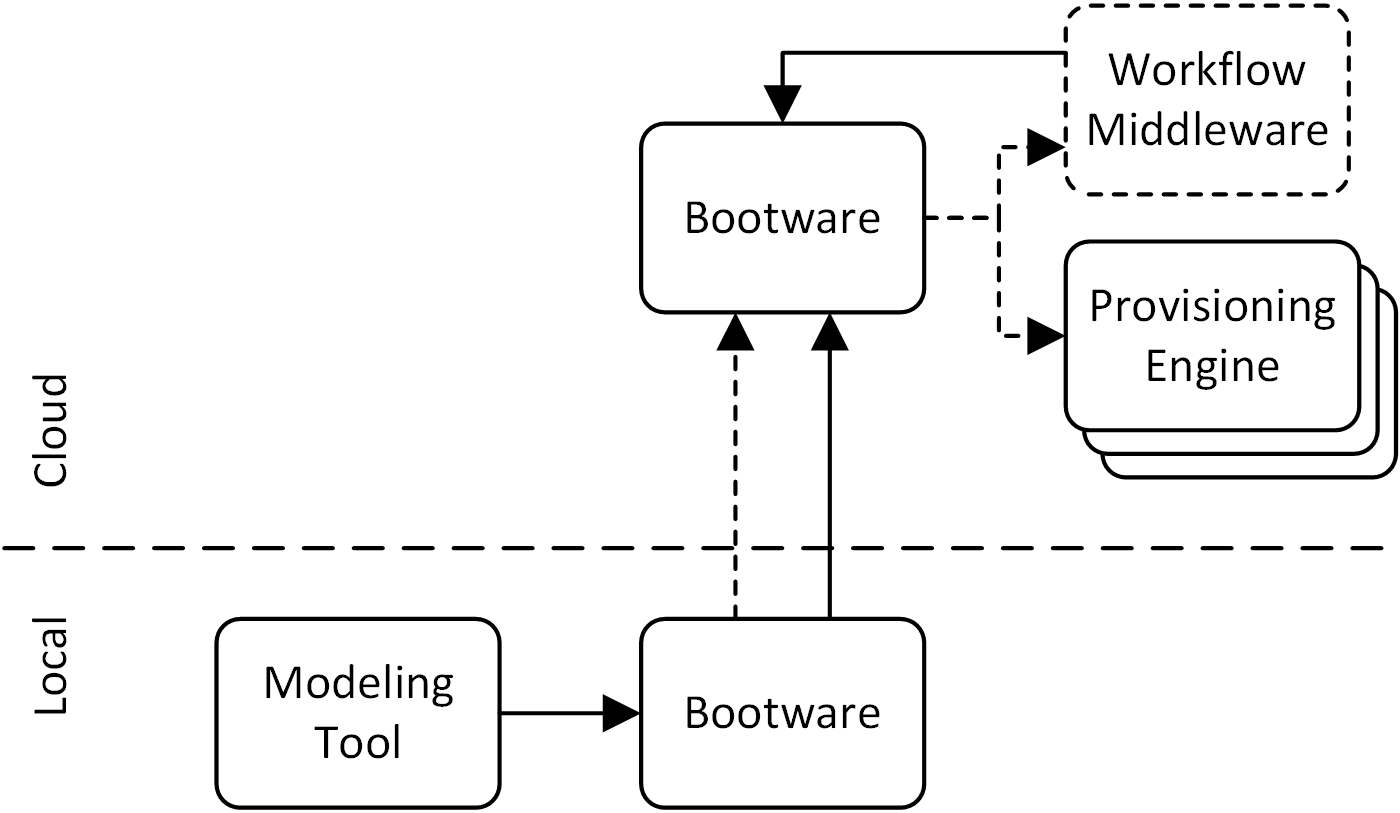
\includegraphics[resolution=600]{design/assets/simple_clone}
	\caption{Simplified overview of the cloned component architecture}
	\label{image:clone}
\end{figure}

This architecture can be seen as an alternative form of the 2-tier architecture described in \autoref{design:division:2tier}.
In this case there are also two parts working together and the remote part does most of the work.
However, the local and the remote components are identical.
Instead of provisioning a bigger component in a remote environment, the local component clones itself.
Compared to the 2-tier architecture described before, this has the advantage that only one component has to be designed and implemented and that function duplication is not an issue.
On the other hand, this architecture makes only sense if the functionality of the two separate components in the 2-tier architecture turns out to be mostly identical.
Therefore we can't decide yet if this architecture should be used.

\subsubsection{Decision}

Of the four alternative presented here, alternative three - the 2-tier architecture - makes the most sense.
Therefore it is selected as the alternative of choice and used for further discussion.
We do however retain the option to transform it into alternative four if this seems advantageous.

\subsection{Extensibility}
\label{design:extensibility}

The requirements for the bootware component state that support for different cloud environments and provisioning engines should be achieved through means of software engineering.
This requirement is intentionally vague to allow to select a fitting extension mechanism during the design process.

\subsubsection{Extension Mechanisms}

\textcolor{red}{other mechanisms?}

One possibility that would satisfy this criteria is to design interfaces for all extension points of the bootware component.
New cloud environments, provisioning engines, or other extension could then implement these interfaces.
The disadvantage of this approach is that the whole bootware component has to be recompiled, redistributed and redeployed if one extension is added or changed.

To remove this disadvantage, a more flexible architecture is needed, for example a plugin architecture. (\textcolor{red}{pattern?})
Interfaces for the extension points still exist but the extension are no longer part of the main bootware component.
They are compiled separately into plugins that can be loaded into the main bootware component on the fly.
There are several possibilities to realize such an architecture.

It is certainly possible to implement a plugin framework from scratch.
An advantage of this approach would be that the design of the plugin architecture could be tailored to our use case and would be as simple or complex as needed.
But there are also several disadvantages.
For one, we would reinvent the wheel, since multiple such frameworks already exist.
It would also shift resources away from the actual goal of this thesis, which is designing the bootware component.
Furthermore it would require a deep understanding of the language used for the implementation (\textcolor{red}{in this case Java}), which is not necessarily given.
Therefore it seems more reasonable to use one of the already existing plugin frameworks.Three such alternatives will be compared next. (\textcolor{red}{more?})

\subsubsection{Plugin Frameworks}

\begingroup
	\centering
	\captionsetup{type=table}
	\begin{tabu}[!htbp]{rl|[0.5pt]ccc}

		&
		& \multicolumn{3}{c}{\textit{Plugin Frameworks}} \\

		&
		& \begin{sideways} \textbf{JSPF\footnote{\url{https://code.google.com/p/jspf/}\label{jspf}}} \end{sideways}
		& \begin{sideways} \textbf{JPF\footnote{\url{http://jpf.sourceforge.net/}\label{jpf}}} \end{sideways}
		& \begin{sideways} \textbf{OSGi\footnote{\url{http://www.osgi.org/}\label{osgi}}} \end{sideways} \\

		\tabucline[0.5pt]{2-5}

		\multirow{7}{*}{\textit{Features}}

		& \textbf{Security}
		& \ding{55}    % jspf
		& \ding{55}    % jpf
		& \ding{51} \\ % osgi

		& \textbf{Dynamic Loading}
		& \ding{55}    % jspf
		& \ding{51}    % jpf
		& \ding{51} \\ % osgi

		& \textbf{Complexity}
		& low     % jspf
		& medium  % jpf
		& high \\ % osgi

		& \textbf{Active Development}
		& \ding{55}    % jspf
		& \ding{55}    % jpf
		& \ding{51} \\ % osgi

		& \textbf{Popularity}
		& low     % jspf
		& low     % jpf
		& high \\ % osgi

		& \textbf{Standard}
		& \ding{55}    % jspf
		& \ding{55}    % jpf
		& \ding{51} \\ % osgi

		& \textbf{Used in SimTech}
		& \ding{55}    % jspf
		& \ding{55}    % jpf
		& \ding{51} \\ % osgi

		\tabucline[0.5pt]{2-5}

	\end{tabu}
	\caption{Feature comparison of Java plugin frameworks}
	\label{table:plugin_comparison}
\endgroup

All of the frameworks that we compare here offer the basic functionality that we need to extend the core bootloader component, i.e. the developer defines interfaces that then are implemented by one or more plugins.
These plugins are compiled separately from the main component and are then packaged in \textit{.jar} files for distribution.
These packages are loaded during runtime and provide the implementation for the specific interface they implement.
There are however some advanced functional differences and some non-functional differences that will be considered here.

Dynamic loading allows us to load and replace plugins during runtime, without completely restarting the application.
While we don't know for certain if dynamic loading is needed in our case, it's one of the advanced features that might be nice to have in the future.

Security is a must have feature but is out of the scope of this thesis.
Consider the following scenario: The bootware component is used by multiple separate users who can share plugins using a plugin repository.
Without security features, a malicious user could upload a plugin to this repository which, in theory, could contain any code.
Therefore it's important to select the right framework now, so that security features can be implemented in the future.

Some non-functional features should also be considered, such as complexity, popularity, and if the framework is still in active development.

\nom{Java Simple Plugin Framework}{JSPF}\footref{jspf} is a plugin framework build for small to medium sized projects.
Its main focus is simplicity.
Therefore it does not support many of the advanced features like dynamic loading or security that other solution support.
The author explicitly states that it is not intended to replace JPF or OSGi~\autocite{jspf:faq}.

\nom{Java Plugin Framework}{JPF}\footref{jpf} is an open-source plugin framework.
Compared to JSPF it supports some advanced features like dynamic loading of plugins during runtime.
It is also more popular then JSPF.
However, the last version was released in 2007.
This is not necessarily bad but might show that there will be no future development of this framework.

\nom{Open Service Gateway initiative}{OSGi}\footref{osgi} is a plugin framework standard developed by OSGi Alliance.
It provides a general-purpose Java framework that supports the deployment of extensible bundles~\autocite{osgi:spec}.

\textcolor{red}{Decision}

\subsubsection{Plugin Repository}

Now that we have introduced plugins we face new problems.
\autoref{image:plugins} shows the current architecture, where both bootware components use their own plugins.
If a plugin is added or updated, the user has to manually copy this plugin to the right folder of one or both of the bootware components.
Furthermore, if both components use the same plugins, which they will (cloud plugins), we will have duplicate plugins scattered around.
This is inefficient, probably annoying for the user and possibly dangerous (\textcolor{red}{other world, fehler hervorrufend}) if plugins get out of sync.

\begin{figure}[!htbp]
	\centering
	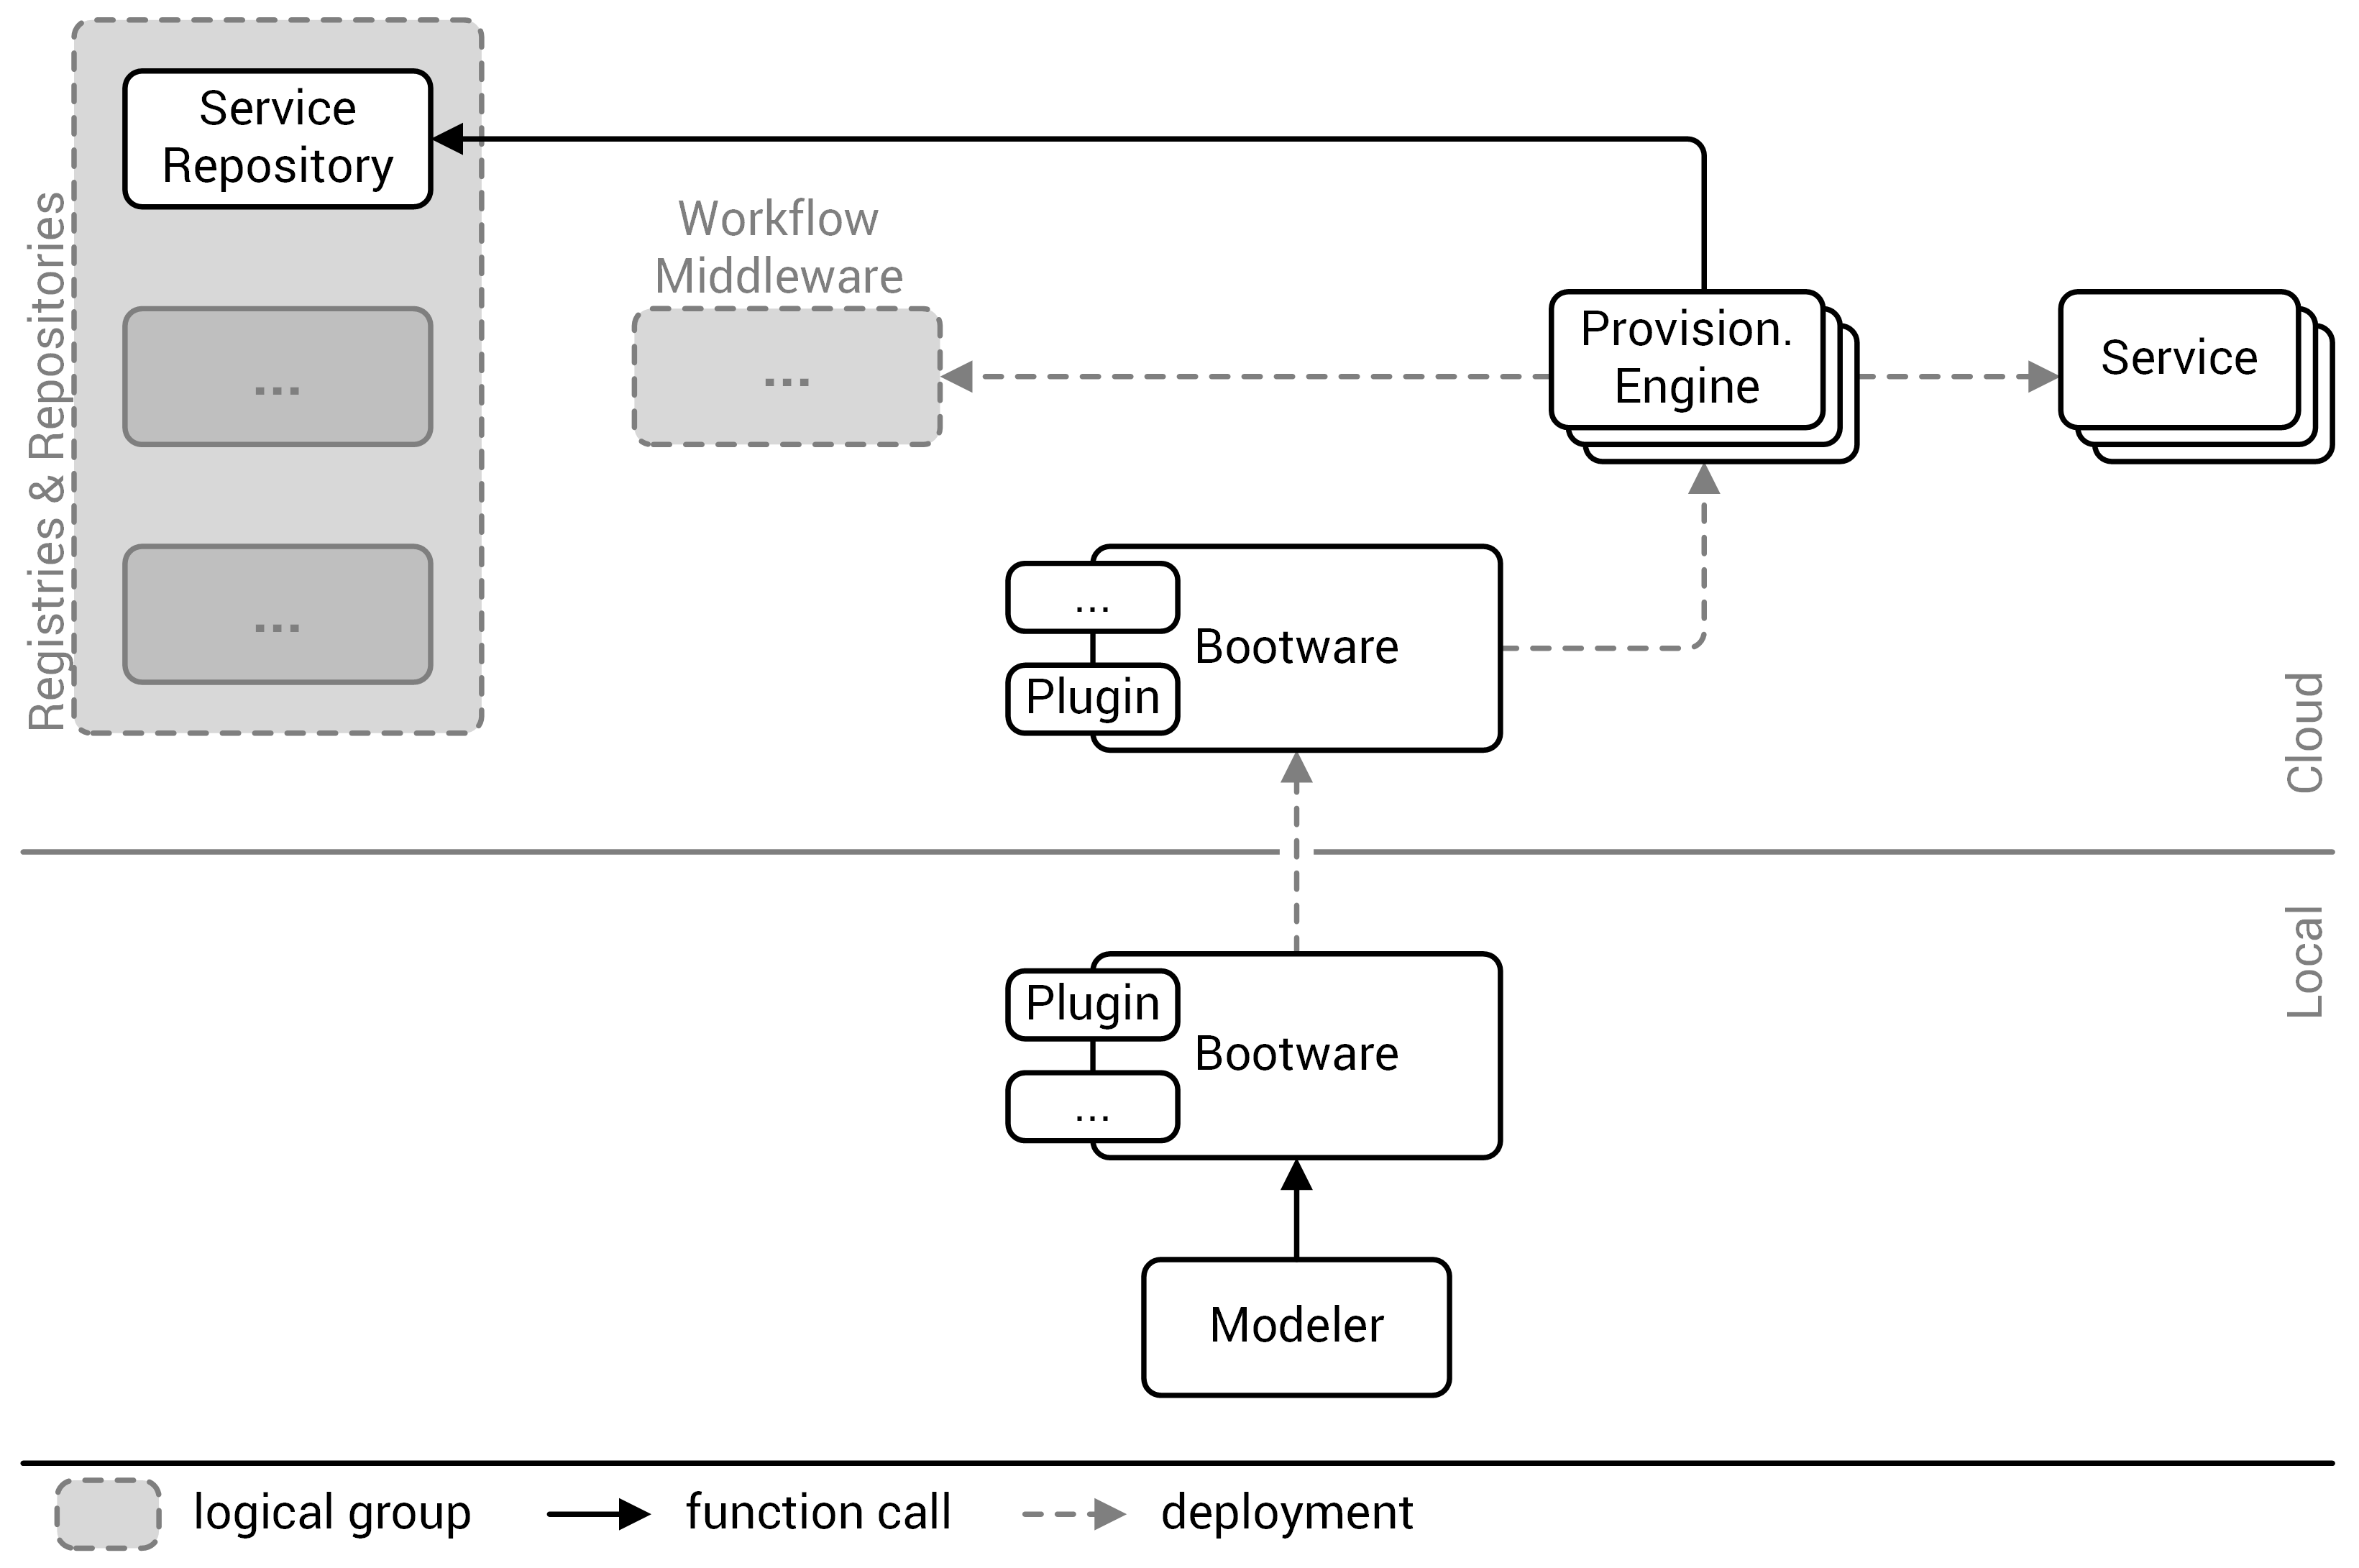
\includegraphics[resolution=600]{design/assets/simple_plugins}
	\caption{Simplified overview of the 2-tier architecture with plugins}
	\label{image:plugins}
\end{figure}

To remedy this situation we introduce a central plugin repository, as shown in \autoref{image:plugin_repository}.
This repository holds all plugins of both components so it eliminates duplicate plugins.
If plugins are added or modified it has only to be done in one place.
Plugin synchronization can happen automatically when the bootware components start, so that the user is no longer involved in plugin management.
The repository also enables easy plugin sharing, which was cumbersome earlier.

\begin{figure}[!htbp]
	\centering
	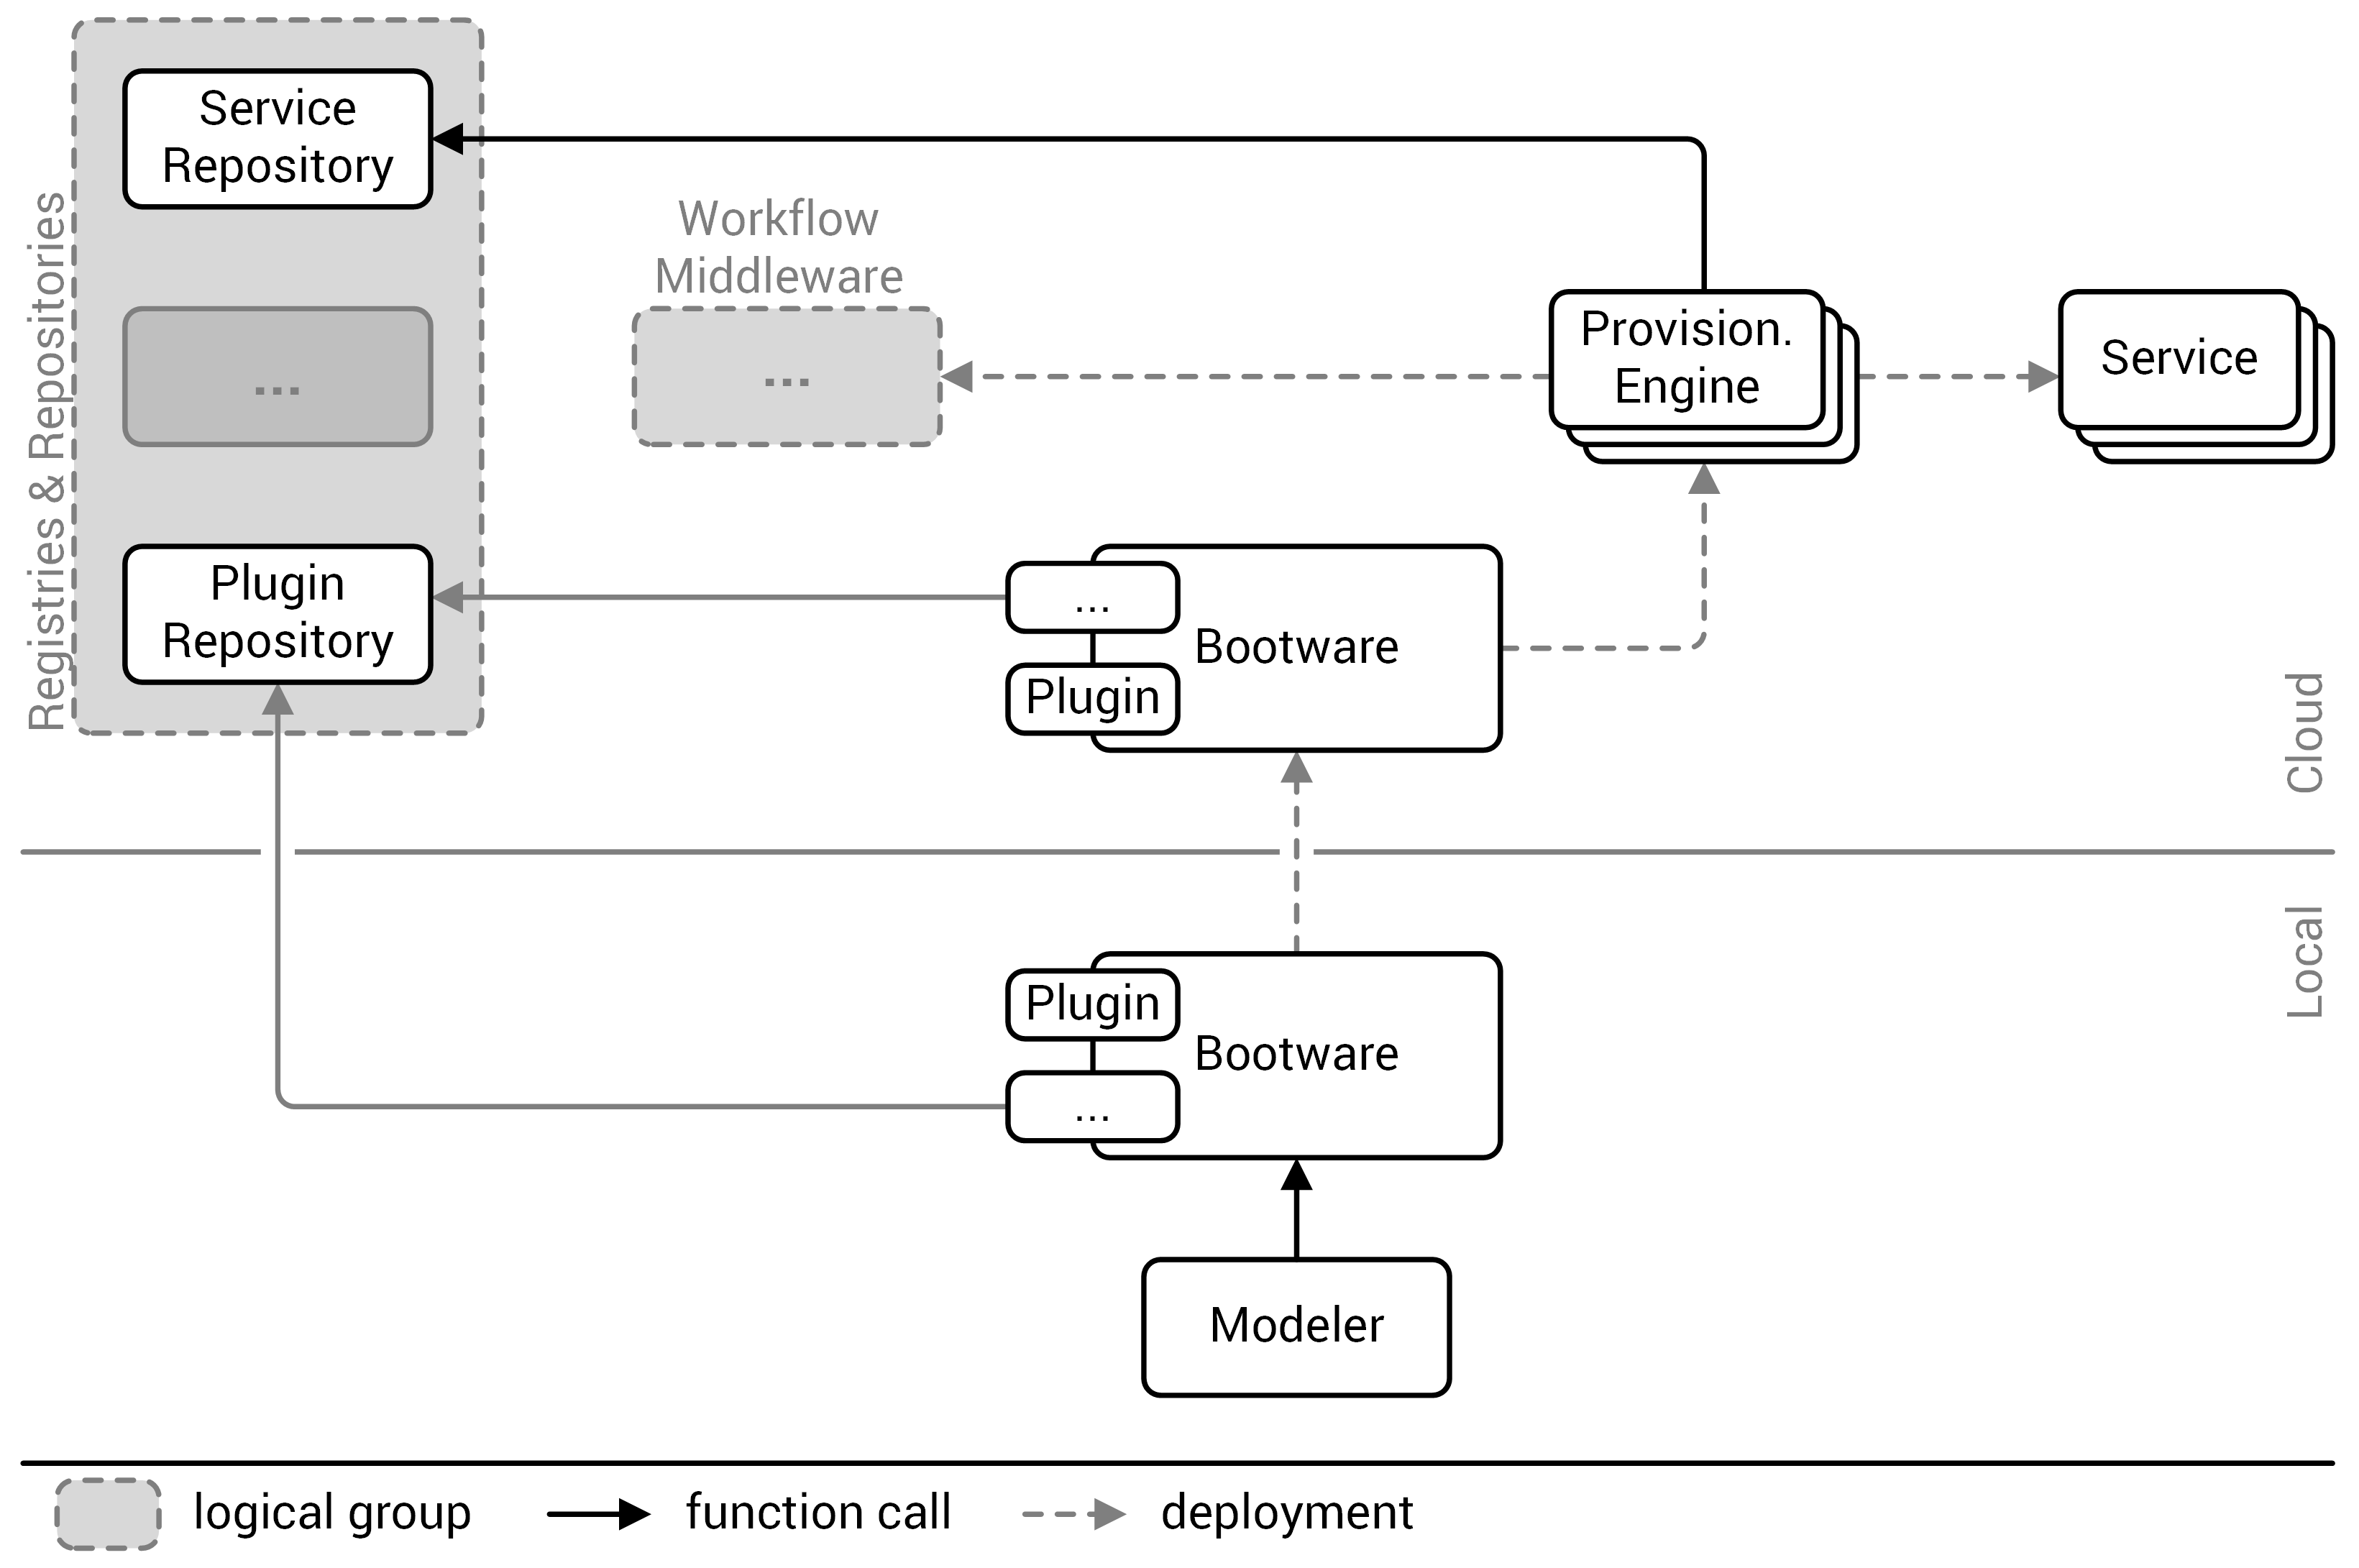
\includegraphics[resolution=600]{design/assets/simple_plugin_repository}
	\caption{Simplified overview of the 2-tier architecture with a plugin repository}
	\label{image:plugin_repository}
\end{figure}

While a central plugin repository is a sensible addition to the proposed bootware architecture, its design and implementation are out of scope of this thesis.

\subsection{Communication}
\label{design:communication}

Since we will use a 2-tiered approach for the bootware component, we now have to decide, how the communication between the two components will work.
There are several factors that impact this decision.

Communication between the components should be as simple as possible, but has to support some critical features.

Since the provisioning processes kicked off by the bootware can potentially take a lot of time to finish (in the range of minutes to hours), asynchronous communication should be used between the components to avoid timeouts and blocking resources.

For the same reason, there should be some mechanism to get feedback on the current status during a long running provisioning process.

There will be other components that have to call the bootware to start some provisioning process, so communication has to be open for other parties.

The communication with the bootware components will contain sensitive data, for example login information for cloud providers that the bootware needs to do its job, but has to be provided from the outside on a call to call basis.
This information has to be transported securely to prevent malicious or fraudulent attacks.
The selected communication method therefore has to support some sort of security mechanisms, ideally end-to-end security via message encryption.
While these security mechanisms will not be used in this thesis due to time constraints, selecting the right communication method is still critical for future development.

Since this whole project is concerned with services, it \textcolor{red}{liegt nahe} to use web service calls and returns as main communication method, internally as well as  externally.
This way we offer a consistent interface for all components to use.
\autoref{image:webservice} shows the addition of asynchronous web service call and return communication to the proposed architecture.
Using a web service with soap messaging also gives us access to Web Service Security Framework, which supports end-to-end security with encryption and signatures.

\begin{figure}[!htbp]
	\centering
	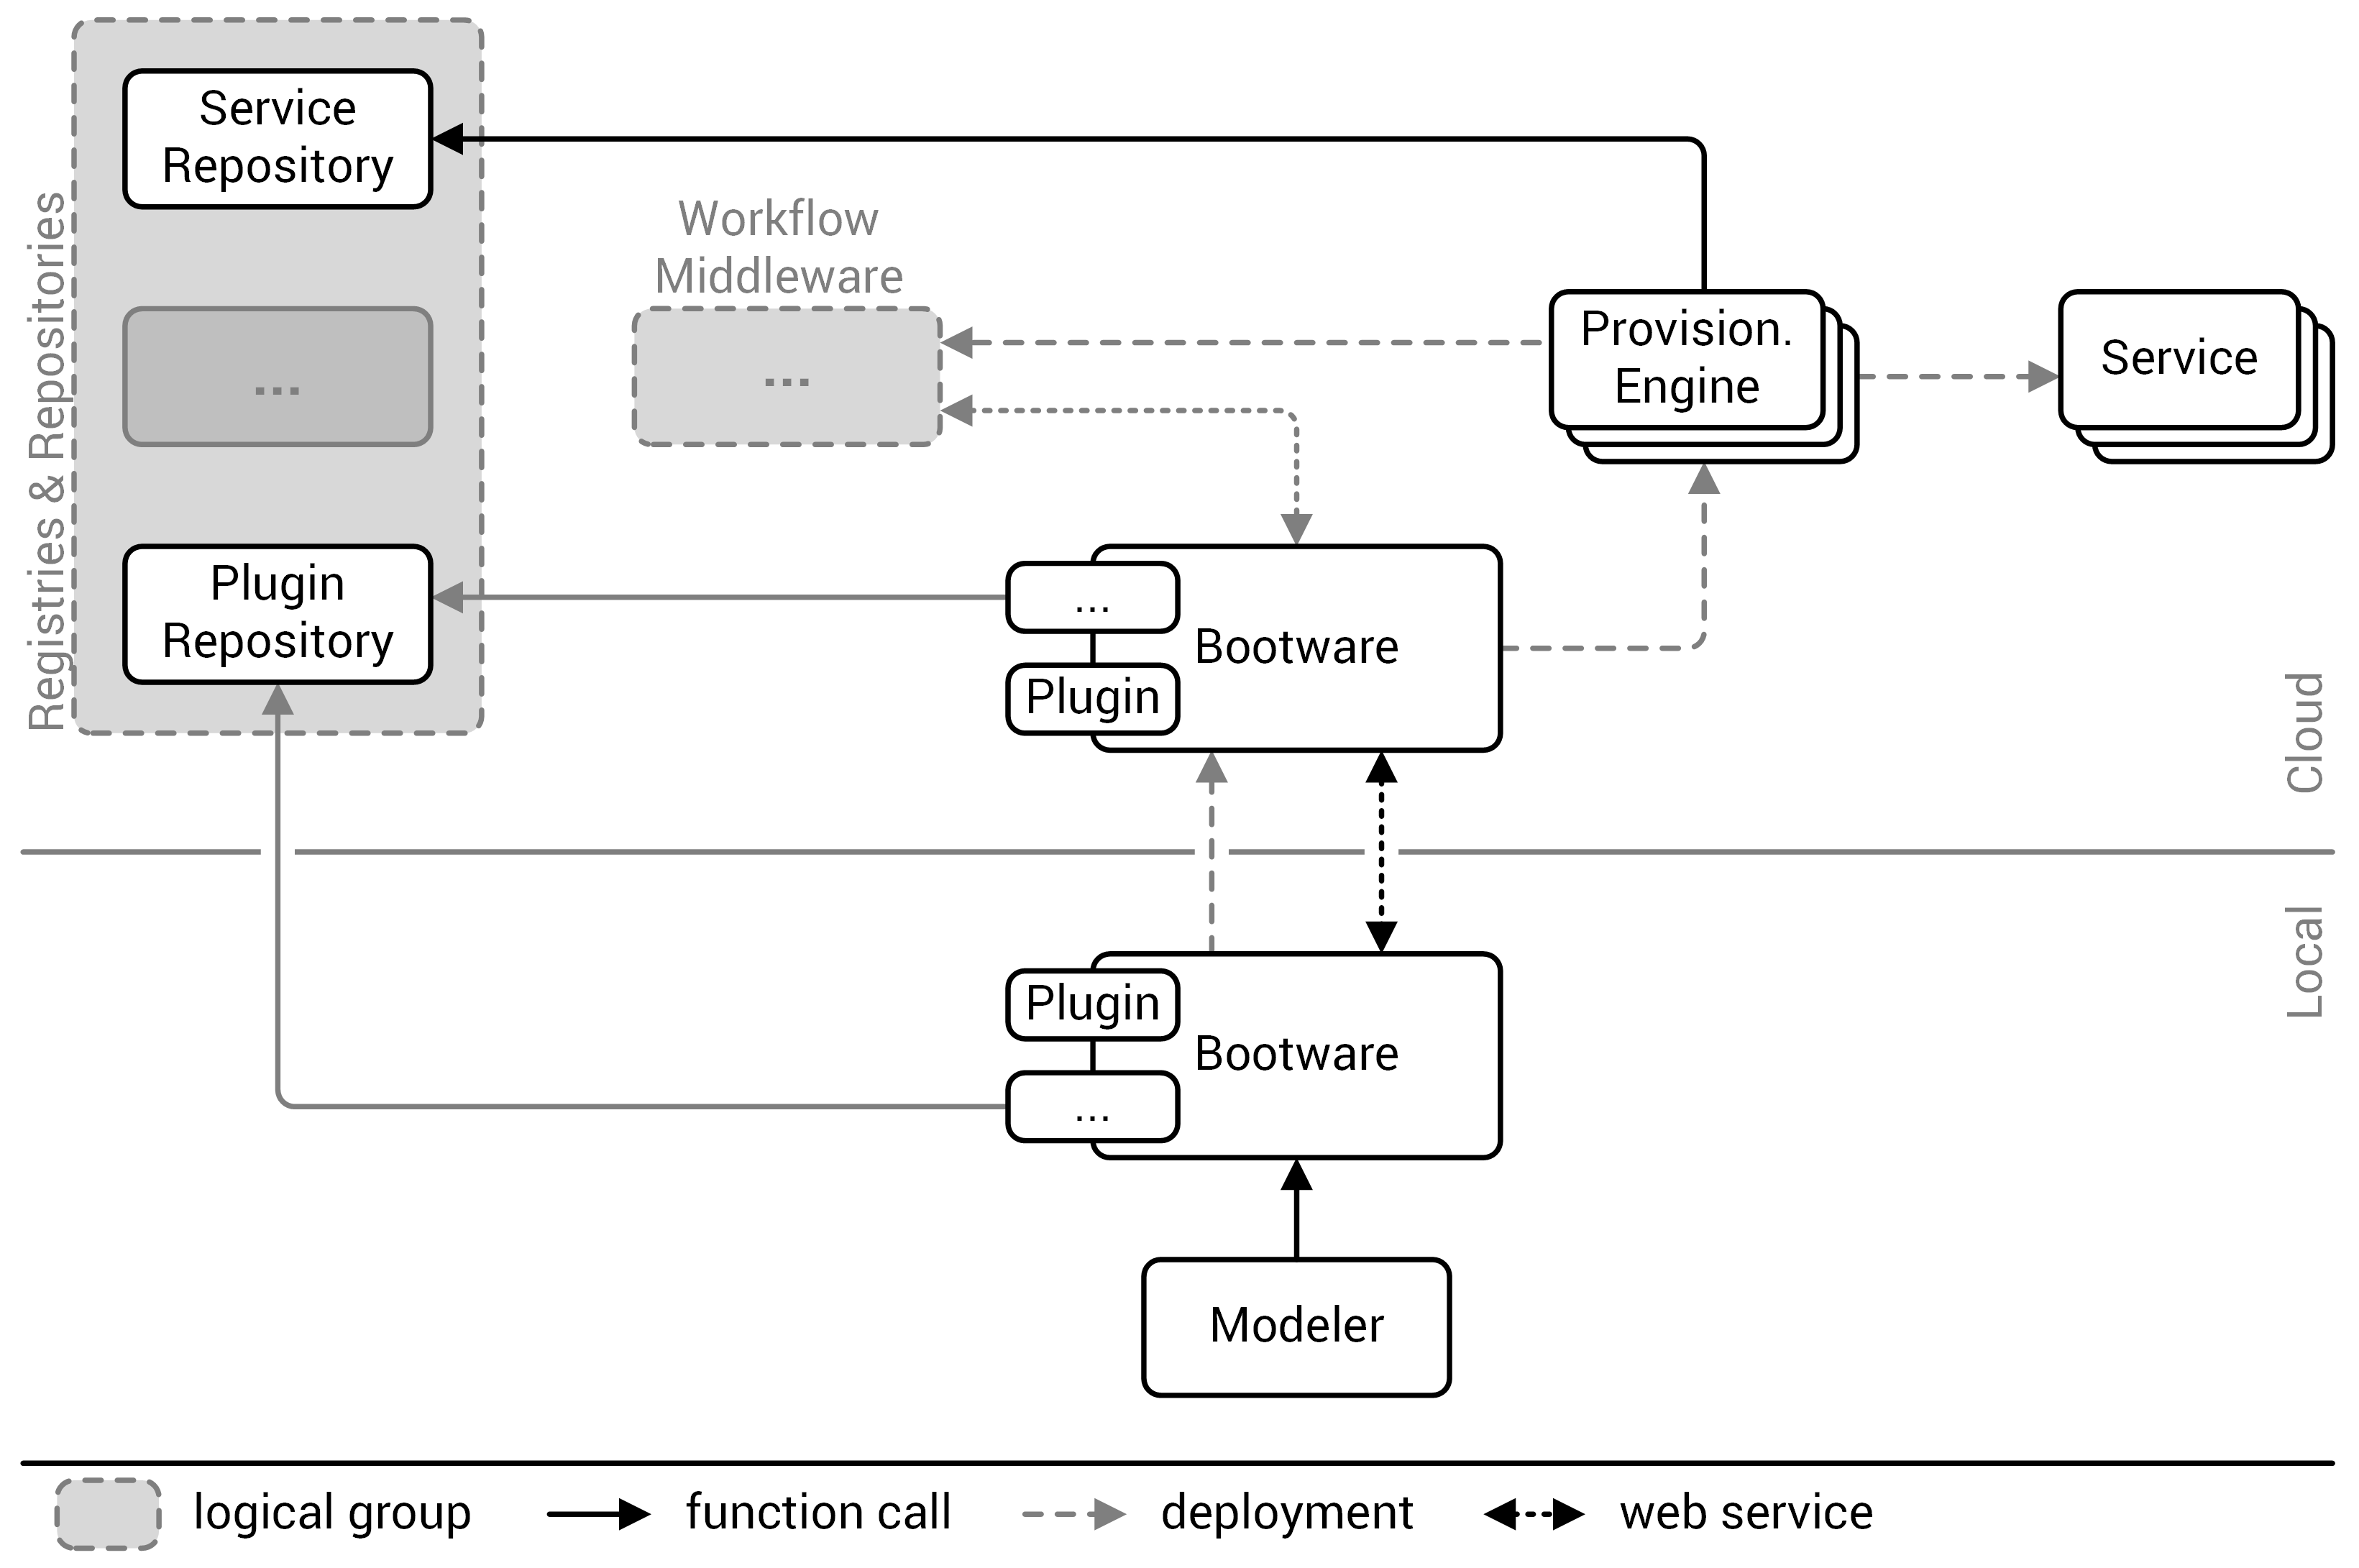
\includegraphics[resolution=600]{design/assets/simple_webservice}
	\caption{Simplified overview of the 2-tier architecture with asynchronous web service communication}
	\label{image:webservice}
\end{figure}

Web Services also support asynchronous communication so that long running provisioning processes won't pose a problem.
We do however still need information during those long running processes to give the user some feedback.
This can't (\textcolor{red}{???}) be accomplished by this simple request/response pattern.
For this, a secondary communication mechanism which supports sending multiple feedback messages has to be used.

Since it is not necessary for the successful use of the bootware it would make sense to implement this secondary communication mechanism as a plugin.
This would allow us to add arbitrary communication plugins to the bootware depending on future needs.

One natural choice for this is the PubSub pattern implemented by some messaging middleware.
Using this pattern, the remote bootware component pushes messages to a message queue to which the local bootware component (and other components if needs be) can subscribe to receive future messages.
\autoref{image:queue} shows an additional message queue.

\begin{figure}[!htbp]
	\centering
	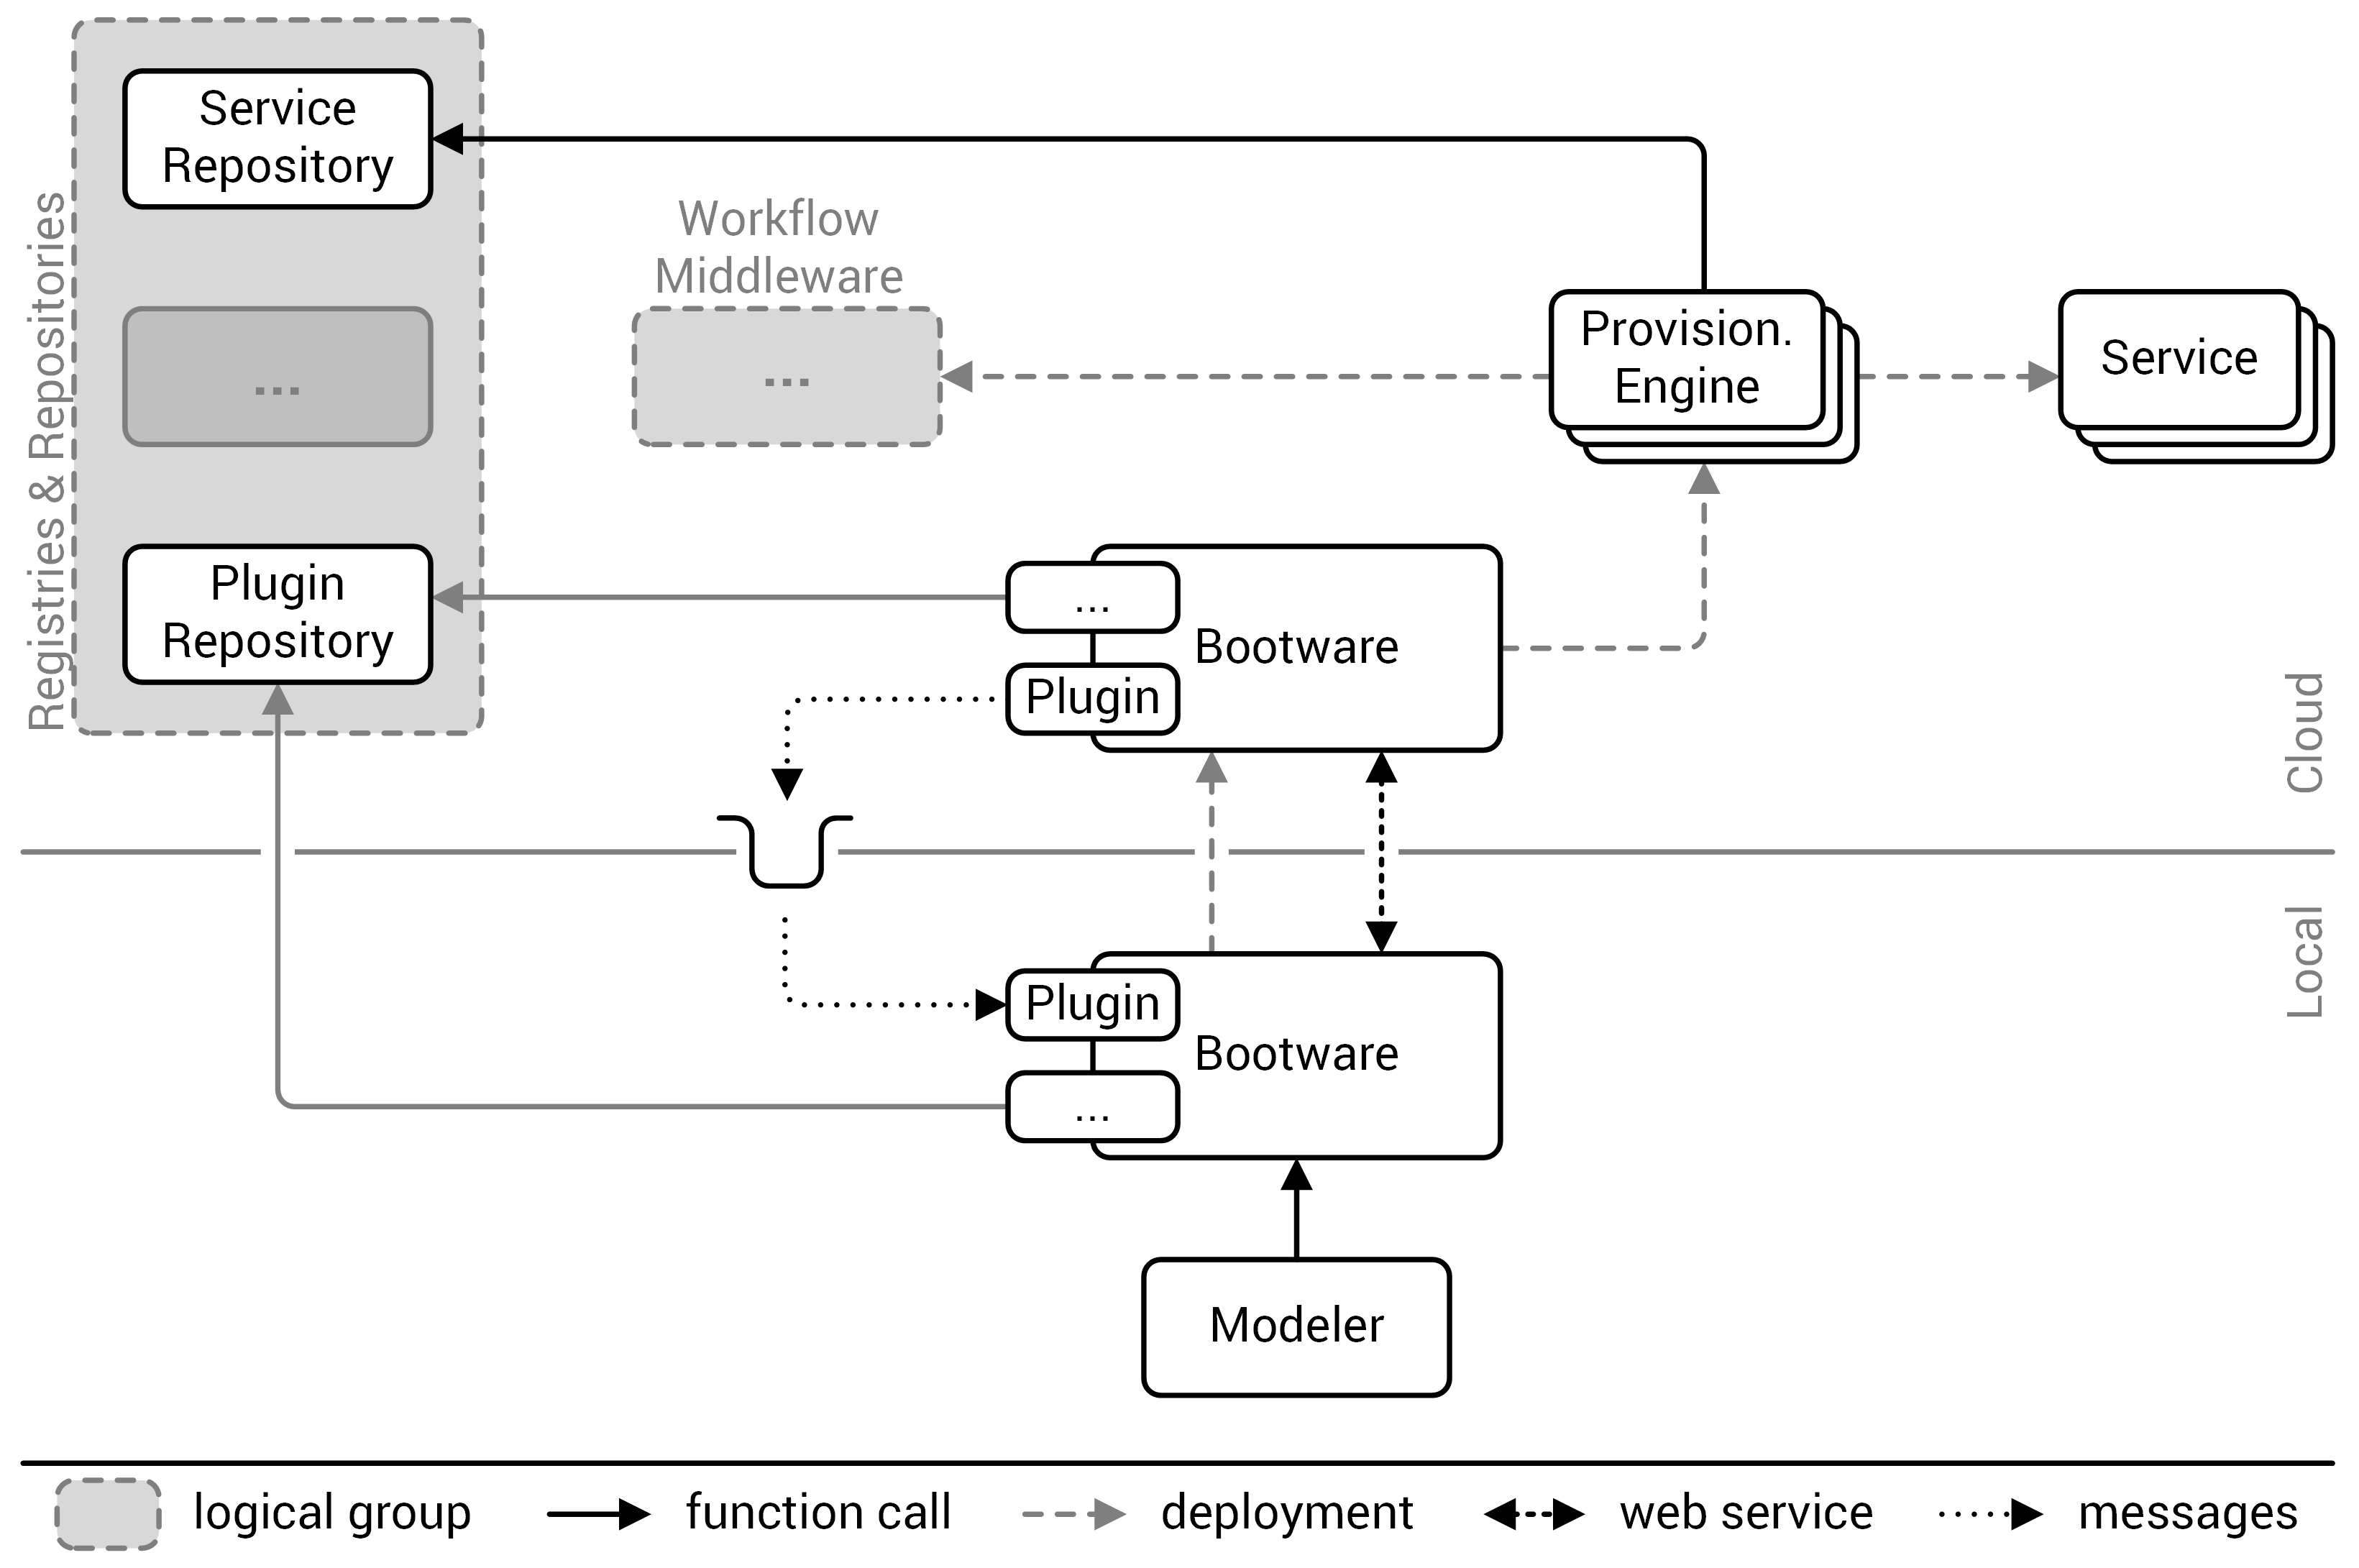
\includegraphics[resolution=600]{design/assets/simple_queue}
	\caption{Simplified overview of the 2-tier architecture with asynchronous web service and a messaging queue communication}
	\label{image:queue}
\end{figure}

\subsection{Internal Communication}

We also have to consider internal communication between the bootware core and plugins, and possibly also in between plugin.
Ideally, every plugin will be able to react to events from the bootware.
These event could be triggered by the bootware core or by any plugin, but plugins should be completely independent from each other.
Since a plugin doesn't know about other plugins, it can't listen for events at other plugins directly.
The only known constant to a plugin is the bootware core.
Therefore we need a communication mechanism which allows for loosely coupled communication between the bootware core and the plugins, where plugins can register their interest for certain events with the core and also publish their own events to the core for other plugins to consume.
This essentially describes the publish-subscribe pattern (\textcolor{red}{ref}).

\subsubsection{PubSub}

The \nom{publish-subscribe pattern}{PubSub} is a messaging pattern that consists of three types of participant who aren't necessarily mutually exclusive: Event busses (or message broker), publishers, and subscribers.
The event bus sits at the center of the communication.
He receives messages from publishers and distributes them to all subscribers that have voiced their interest in messages of a certain type by subscribing at the event bus.

Using this pattern in our bootware component, we would create an event bus at the bootware core and plugins, as well as other parts of the core, could subscribe at this event bus and also publish messages through this event bus.

\subsubsection{PubSub Libraries}

Many of the well know Messaging Middlewares offer support for PubSub, for example \textcolor{red}{ActiveMQ,...}.
But, since we are looking for an internal communication mechanism only, all of these solutions are somewhat overpowered.
We don't need \textcolor{red}{guaranteed delivery, message queuing, scalability,...}.
Instead, we need a lightweight in-memory solution.
Therefor we will ignore the middleware heavyweights and look for smaller, more light weight PubSub libraries.

\begingroup
	\centering
	\captionsetup{type=table}
	\begin{tabu}[!htbp]{rl|[0.5pt]ccccc}

		&
		& \multicolumn{5}{c}{\textit{PubSub Libraries}} \\

		&
		& \begin{sideways} \textbf{MBassador\footnote{\url{https://github.com/bennidi/mbassador}\label{mbassasor}}} \end{sideways}
		& \begin{sideways} \textbf{Guava Event Bus\footnote{\url{https://code.google.com/p/guava-libraries/wiki/EventBusExplained}\label{guava}}} \end{sideways}
		& \begin{sideways} \textbf{Simple Java Event Bus\footnote{\url{https://code.google.com/p/simpleeventbus/}\label{simpleeventbus}}} \end{sideways}
		& \begin{sideways} \textbf{EventBus\footnote{\url{http://eventbus.org/}\label{eventbus}}} \end{sideways}
		& \begin{sideways} \textbf{Mycila PubSub\footnote{\url{https://github.com/mycila/pubsub}\label{mycilapubsub}}} \end{sideways} \\

		\tabucline[0.5pt]{2-7}

		\multirow{1}{*}{\textit{Features}}

		& \textbf{Something}
		& \ding{55}    % mbassador
		& \ding{55}    % guava
		& \ding{51}    % simpleeventbus
		& \ding{51}    % eventbus
		& \ding{51} \\ % mycila

		\tabucline[0.5pt]{2-7}

	\end{tabu}
	\caption{Feature comparison of Java PubSub libraries}
	\label{table:pubsub_comparison}
\endgroup
